\documentclass{svproc}
\usepackage{graphicx}
\usepackage{multicol}
\usepackage{footmisc}
\usepackage{amstext}
\usepackage{amsmath}
\usepackage{amssymb}
\usepackage[english]{babel}
\usepackage[official,right]{eurosym}
\selectlanguage{english}
% Ampersand -----------------------------------------------------------

\def\id#1{\text{\em #1\/}}
\newcommand{\code}[1]{\text{\tt\small #1}}
\newcommand{\stmtText}[1]{``{\small\tt #1}''}
\newcommand{\dom}[1]{\id{dom}(#1)}
\newcommand{\cod}[1]{\id{cod}(#1)}
\renewcommand{\int}[2]{\id{inter}(#1,#2)}
\newcommand{\pop}[1]{\id{pop}(#1)}
\newcommand{\src}[1]{\id{src}(#1)}
\newcommand{\trg}[1]{\id{trg}(#1)}
\newcommand{\powerset}[1]{\cal{P}\{#1\}}
\newcommand{\theCode}{\url{http://cs.ru.nl/~B.Joosten/ampTypes/}}
\newcommand{\la}{\langle}
\newcommand{\ra}{\rangle}
\newcommand{\full}{V}
\newcommand{\declare}[3]{\id{#1}_{\pair{\id{\small #2}}{\id{\small #3}}}}
\newcommand{\fullt}[2]{V_{\pair{#1}{#2}}}
\newcommand{\iden}[1]{I}
\newcommand{\ident}[1]{I_{\id{\small #1}}}
\newcommand{\expr}[3]{(#1)_{#2\times #3}}
\newcommand{\pair}[2]{\la{#1},{#2}\ra}
\newcommand{\atom}[1]{{\tt\small #1}}
\newcommand{\atoms}{\mathcal{A}}
\newcommand{\concepts}{\mathcal{C}}
\newcommand{\decls}{\mathcal{D}}  %% names of relations
\newcommand{\rels}{\mathcal{R}}   %% all relations
\newcommand{\relations}{\mathcal{M}} % representing terms. M is a subset of R.
\newcommand{\terms}{\mathcal{T}}
\newcommand{\vertices}{N}
\newcommand{\rules}{\mathcal{H}}
\newcommand{\tf}[1]{\mathfrak{T}(#1)}
\newcommand{\ptf}[1]{\mathfrak{T}'(#1)}
\newcommand{\ti}[1]{\mathfrak{I}(#1)}
\newcommand{\tic}[1]{I_{\cal C}(#1)}
\newcommand{\relAdd}{\dagger}
\newcommand{\flip}[1]{{#1}^\smallsmile} %formerly:  {#1}^\backsim
\newcommand{\kleeneplus}[1]{{#1}^+}
\newcommand{\kleenestar}[1]{{#1}^*}
\newcommand{\cmpl}[1]{\overline{#1}}
\newcommand{\rel}{\times}
\newcommand{\compose}{;}
\newcommand{\subs}{\subseteq}%{\models}
\newcommand{\fun}{\rightarrow}
\newcommand{\isa}{\preceq}
%\newcommand{\isaClos}{\sqsubseteq}
\newcommand{\typetest}{?}
\newcommand{\meet}{\sqcap}
\newcommand{\join}{\sqcup}
\newcommand{\Meet}{\bigsqcap}
\newcommand{\Moin}{\bigsqcup} % because LaTeX has already defined command \Join.
\newcommand{\order}{\ominus}
\newcommand{\anything}{\top}
\newcommand{\nothing}{\bot}
\newcommand{\rewriteto}{\rightarrow}
\newcommand{\calc}{\implies}
\newcommand{\alland}{\bigwedge}
\newcommand{\mph}[3]{#1_{#2\times #3}}
\newcommand{\mphu}[1]{#1_{\univ\times\univ}}

%-----------------------------------------
\newcommand{\kse}{\hspace*{1.7em}}
\newcommand{\ksf}{\hspace*{1em}}
\newcommand{\ksg}{\hspace*{1em}}
\newenvironment{derivation}{\begin{tabbing}\kse \= \ksf \= \ksg \= \kill}{\end{tabbing}}
\newtheorem{definition}{Definition}
\newcommand{\term}[1]{\>\>\(#1\)\\[1ex]}
\newcommand{\rela}[2]{\>\(#1\)\>\>\{ \ #2 \ \}\\[1ex]}
\newcommand{\weg}[1]{}

\def\define#1{\label{dfn:#1}{\em #1}\index{#1}}
\def\definem#1{\label{dfn:#1}{\em #1}\index{#1}\marge{#1}}
\newcommand{\marg}[1]{\index{#1}\marge{#1}}

\begin{document}

\title{Software Development in Relation Algebra with Ampersand}
\toctitle{Software Development in Relation Algebra with Ampersand}
%\titlerunning{Ampersand} % (for running head)
\author{Stef Joosten\inst{1,}\inst{2} (0000-0001-8308-0189)}
%orcid.org/0000-0001-8308-0189
\authorrunning{Stef Joosten} % (for running head)
\tocauthor{Stef Joosten} % for table of contents
\institute{Open Universiteit Nederland,\\  Postbus 2960,   6401 DL Heerlen, the Netherlands\\
\and Ordina NV,  Nieuwegein, the Netherlands\\
\email{stef.joosten@ou.nl} % optional, same for URL of homepage
} % end of address field
\maketitle

\abstract{Relation Algebra can be used as a programming language for building information systems.
	This paper presents a case study to demonstrate this principle.
	We have developed a database-application for legal reasoning as a case study,
	of which a small part is discussed in this paper to illustrate the mechanisms of programming in Relation Algebra.
	Beside being declarative, relation algebra comes with attractive promises for developing big software.
	The compiler that was used for this case study, Ampersand, is the result of an open source project.
	Ampersand has been tried and tested in practice and is available as free open source software.
\keywords{relation algebra, software development, legal reasoning, information systems design, Ampersand, MirrorMe, big software}
	}% abstract contains 102 words

\section{Introduction}
\label{sct:Introduction}
	This paper investigates how relation algebra can be used as a programming language for information systems.
	A compiler, Ampersand~\cite{Michels2011}, is used to compile concepts, relations and rules into a working database-application.
	Ampersand is a syntactically sugared version of heterogeneous relation algebra \cite{Schmidt1997}.
	We present a case study to demonstrate programming in relation algebra and its impact on the software development process.
	The case study takes the reader by the hand in the thinking process of a software developer who programs with relation algebra.

	The use of relation algebra as a programming language is not new.
	It stands in the tradition of relation algebra~\cite{Maddux06}, logic programming~\cite{Lloyd1984},
	database application programming~\cite{Codd70}, and formal specification of software.
	Ampersand uses these ideas to compile relation algebra to working software, an idea which is also found in RelView~\cite{Berghammer2005} by Berghammer (Univ. of Kiel).
	Some differences with earlier programming languages are discussed in section~\ref{sct:Reflection}, after presenting the case study.
	
	The user may regard Ampersand as a programming language, especially suited for designing the back-end of information systems.
	The axioms of Tarski can be used to manipulate expressions in a way that preserves meaning~\cite{vdWoude2011}.
	This makes Ampersand a declarative language.

	Our case study shows an argument assistant for legal professionals, which was built as innovation project at Ordina.
	The purpose of this argument assistant is to support legal professionals in constructing a legal brief%
\footnote{A \define{brief} is a document that is meant to summarize a lawsuit for the judge and counterparty.
	It provides legal reasons for claims in a lawsuit based on regulations, precedents, and other legally acceptable sources.
	It shows how the reasoning applies to facts from the case.}.
	The challenge is to create a program that consists of relation algebra as much as possible.
	In doing so, we hope to learn more about software development in relation algebra.

	Section~\ref{sct:Ampersand} introduces Ampersand and its computational semantics.
	Section~\ref{sct:Conceptual analysis} introduces a theory of legal reasoning,
	which was developed for argument assistance.
	Section~\ref{sct:Programming in RA} discusses the programming mechanism in the application,
	and section~\ref{sct:Programming} visualizes that mechanism.
	Section~\ref{sct:Reflection} reflects on software development in Ampersand.
	It also provides an overview of the use of Ampersand in practice and an outlook to its further development.

\section{Ampersand}
\label{sct:Ampersand}
	In this section we explain the basics of Ampersand.
	The reader is expected to have sufficient background in relation algebra,
	in order to understand the remainder of this paper.

	The core of an Ampersand-script is a tuple $\la\rules,\rels,\concepts,\mathfrak{T}\ra$, which consists of a set of rules $\rules$, relations $\rels$, concepts $\concepts$, and a type function $\mathfrak{T}$.
	Ampersand-scripts are interpreted by the compiler as an information system.
	The rules constitute a theory in heterogeneous relation algebra.
	They constrain a body of data that resides in a database.
	The Ampersand-compiler generates a database from relations in the script.
	A database-application%
\footnote{Ampersand generates an application that consists of a relational database and interface components.
	Currently this application runs server-side on a PHP/MySQL platform and on a web-browser on the client-side.}
	assists users to keep rules satisfied throughout the lifetime of the database. It is also generated by Ampersand.

	A rule is an equality between two terms.
	Terms are built from relations.
	Ampersand interprets every relation as a finite set of pairs, which are stored in the database.
	The phase in which Ampersand takes a script, and turns it into a database, is what we will refer to as \define{compile-time}.
	The phase in which a user interacts with the database, is what we will refer to as \define{run-time}.
	At run-time, Ampersand can decide which rules are satisfied by querying the database.
	The compiler generates all software needed to maintain rules at run-time.
	If a rule is not satisfied as a result of data that has changed, that change is reverted (rolled back) to
	maintain a state in which all rules are satisfied.
	Changes to the database are not specified by the software developer, but generated by the compiler.
	Rules in Ampersand are maintained rather than executed directly.
	
	Atoms are values that have no internal structure, meant to represent data elements in a database.
	From a business perspective, atoms are used to represent concrete items of the world,
	such as \atom{Peter}, \atom{1}, or \atom{the king of France}.
	By convention throughout the remainder of this paper, variables $a$, $b$, and $c$ are used to represent \emph{atoms}.
	The set of all atoms is called $\atoms$.
        Each atom is an instance of a \emph{concept}.

	Concepts (from set $\concepts$) are names we use to classify atoms in a meaningful way.
	For example, you might choose to classify \atom{Peter} as a person, and \atom{074238991} as a telephone number.
        We will use variables $A$, $B$, $C$, $D$ to represent concepts.
	The term $\ident{A}$ represents the \emph{identity relation} of concept $A$.
	The expression $a \in A$ means that atom $a$ is an instance of concept $A$.
	In the syntax of Ampersand, concepts form a separate syntactic category, allowing a parser to recognize them as concepts.
%	The declaration of $A\isa B$ (pronounce: $A$ is a $B$)
%	in an Ampersand-script states that any instance of $A$ is an instance of $B$ as well.
%	We call this {\em specialization}, but it is also known as {\em generalization} or {\em subtyping}.
	Ampersand also features specialization.
	Specialization is needed to allow statements such as: ``An orange is a fruit that ....''.
	Specialization is not relevant for the remainder of this paper.

	Relations (from set $\rels$) are used in information systems to store facts.
	A \define{fact} is a statement that is true in a business context.
	Facts are stored and kept as data in a computer.
	As data changes over time, so do the contents of these relations.
	In this paper relations are represented by variables $r$, $s$, and $d$.
	We represent the declaration of a relation $r$ by $\declare{nm}{A}{B}$, in which \id{nm} is a name and $A$ and $B$ are concepts.
	We call $A$ the source concept and $B$ the target concept of the relation.
	The term $\fullt{A}{B}$ represents the \emph{universal relation} over concepts $A$ and $B$.

        The meaning of relations in Ampersand is defined by an interpretation function $\mathfrak{I}$.
	It maps each relation to a set of facts.
	Furthermore, it is a run-time requirement that the pairs in $r$ are contained in its type:
\begin{equation}
	\pair{a}{b}\in\ti{\declare{nm}{A}{B}} \Rightarrow\ a \in A \wedge b \in B \label{typing of relations}
\end{equation}

	Terms are used to combine relations using operators.
	The set of terms is called $\terms$. It is defined by:
\begin{definition}[terms]
\label{def:terms}
\item   The set of terms, $\terms$, is the smallest set that satisfies, for all $r,s \in \terms$, $d\in\rels$ and $A,B \in \concepts$: 
\begin{eqnarray}
	d&\in&\terms         \quad\quad\text{(every relation is a term)}\\
	(r \cap s)&\in&\terms\quad\quad\text{(intersection)}\\
	(r-s)&\in&\terms     \quad\quad\text{(difference)}\label{def:difference}\\
	(r;s)&\in&\terms     \quad\quad\text{(composition)}\\
	\flip r&\in&\terms   \quad\quad\text{(converse)}\\
	\ident{A}&\in&\terms \quad\quad\text{(identity)}\\
	\fullt{A}{B}&\in&\terms \quad\quad\text{(full set)}
\end{eqnarray}
\end{definition}
	Throughout the remainder of this paper,	terms are represented by variables $r$, $s$, $d$, and $t$.
	The \define{type} of a term $r$ is a pair of concepts given by $\tf{r}$.
	$\mathfrak{T}$ is a partial function that maps terms to types.
	If term $r$ has a type, this term is called \define{type correct}.
	The Ampersand compiler requires all terms to be type correct, or else it will not generate any code.
	The type function and the restrictions it suffers are discussed in~\cite{Joosten2015}.
	However, for the remainder of this paper this is irrelevant.

    The meaning of terms in Ampersand is an extension of interpretation function $\mathfrak{I}$.
	Let $A$ and $B$ be finite sets of atoms, then $\mathfrak{I}$ maps each term to the set of pairs for which that term stands.
\begin{definition}[interpretation of terms]
\label{interpretation of terms}
\item   For every $A,B\in\concepts$ and $r,s\in\terms$
\begin{eqnarray}
	\ti{r}		 &=&\{\pair{a}{b}|\ a\ r\ b\}	\\
	%\ti{r \cup s}	 &=&\{\pair{a}{b}|\ \pair{a}{b}\in\ti{r}\ \text{or }\ \pair{a}{b}\in\ti{s}\}	\\
	\ti{r \cap s}	 &=&\{\pair{a}{b}|\ \pair{a}{b}\in\ti{r}\ \text{and}\ \pair{a}{b}\in\ti{s}\}	\\
	\ti{r-s}	 &=&\{\pair{a}{b}|\ \pair{a}{b}\in\ti{r}\ \text{and}\ \pair{a}{b}\notin\ti{s}\}	\\
	\ti{r;s}	 &=&\{\pair{a}{c}|\ \text{for some}\ b,\ \pair{a}{b}\in\ti{r}\ \text{and}\ \pair{b}{c}\in\ti{s}\}	\\
	\ti{\flip{r}}	 &=&\{\pair{b}{a}|\ \pair{a}{b}\in\ti{r}    \}	\\
	\ti{\ident{A}} 	 &=&\{\pair{a}{a}|\ a\in A\}	\\
	\ti{\fullt{A}{B}}&=&\{\pair{a}{b}|\ a\in A, b\in B\}
\end{eqnarray}
\end{definition}
	Ampersand has more operators than the ones introduced in definition~\ref{interpretation of terms}:
	the complement (prefix unary $-$),
	Kleene closure operators (postfix $\kleeneplus{\ }$ and $\kleenestar{\ }$),
	left- and right residuals (infix $\backslash$ and $/$),
	relational addition (infix $\dagger$),
	and product (infix $\times$).
	These are all expressible in the definitions above,
	so we have limited this exposition to the operators introduced above.

	The complement operator is defined by means of the binary difference operator (Equation~\ref{def:difference}).
\begin{equation}
	\tf{r}=\pair{A}{B}\ \Rightarrow\ \cmpl{r}\ =\ \fullt{A}{B}-r
\label{eqn:complement}
\end{equation}
	This definition is elaborated in~\cite{vdWoude2011}.

	A \define{rule} is a pair of terms $r,s\in\terms$ with $\tf{r}=\tf{s}$, which is syntactically recognizable as a rule.
\[\text{RULE}\ r = s\]
	This means \(\ti{r} = \ti{s}\). In practice, many rules are written as:
\[\text{RULE}\ r\subs s\]
	This is a shorthand for 
\[\text{RULE}\ r\cap s = r\]
	We have enhanced the type function $\mathfrak{T}$ and the interpretation function $\mathfrak{I}$ to cover rules as well.
	If $\tf{r}=\tf{s}$ and $\tf{s}=\pair{A}{B}$:
\begin{eqnarray}
	\tf{\text{RULE}\ r = s}   &=&\pair{A}{B}\\
	\tf{\text{RULE}\ r\subs s}&=&\pair{A}{B}\\
	\ti{\text{RULE}\ r = s}   &=&\ti{\fullt{A}{B}-((s-r)\cup(r-s))}\\
	\ti{\text{RULE}\ r\subs s}&=&\ti{\fullt{A}{B}-(r-s)}
\end{eqnarray}

	We call rule $r$ \define{satisfied} when $\ti{\text{RULE}\ r = s}\ =\ \ti{\fullt{A}{B}}$.
	As the population of relations used in $r$ changes with time, the satisfaction of the rule changes accordingly.
	A software developer, who conceives these rules, must consider how to keep each one of them satisfied.
	We call a rule \define{violated} if it is not satisfied.
	The set $\ti{(s-r)\cup(r-s)}$ is called the \emph{violation set} of \(\text{RULE}\ r = s\).
	To \define{resolve} violations means to change the contents of relations such that the rule is satisfied%
\footnote{To \define{restore invariance} is sometimes used as a synonym to resolving violations.
	Consequently, a rule is sometimes called \define{invariant}.}.
	Each pair in the violation set of a rule is called a violation of that rule.

	The software developer must define how to resolve violations when they occur.
	She does so by inserting and/or deleting pairs in appropriately chosen relations.
	Whatever choice she makes, she must ensure that her code yields data that satisfies the rules.
	When we say: ``rule $r$ specifies this action'' we mean that satisfaction of rule $r$ is the goal of any action specified by rule $r$. 

\section{Conceptual Analysis}
\label{sct:Conceptual analysis}
	As a case study, an argument assistance system, MirrorMe, was built.
	We have chosen to implement the ideas of Toulmin \cite{Toulmin1958},
	because his book ``The uses of Arguments'' is still one of the most influential works in the area of legal argument management%
\footnote{Thanks to Elleke Baecke for pointing us towards this source.}.
	Toulmin is regarded as the first scholar in modern history to come up with a usable theory of argumentation.
	Recent work typically draws on Toulmin, so his doctrine offers a good starting point.
	Toulmin's ideas have been implemented before, for example in a tool called ArguMed \cite{Verheij1999}.

	Software systems that support legal arguments have been around for many decades.
	Verheij~\cite{Verheij2003} distinguishes between argument assistance systems and automated reasoning systems.
	Automated reasoning has never gained wide acceptance for making legal decisions,
	because lawyers and judges alike feel that human judgment should be at the core of any legal decision.
	Attempts to apply mathematical logic to legal judgments have had limited impact for similar reasons~\cite{Prakken2005}.
	Legal reasoning differs from logic reasoning because of the human judgments that are involved.
	The literature on legal reasoning~\cite{Lind2007} makes it quite clear why mathematical logic alone does not suffice.
	Argument assistance systems~\cite{Verheij2005} have been more successful,
	because they respect the professional freedom of legal professionals to construct their own line of argumentation.
	Such systems offer help in many different ways.
	They can help by looking up legal references, jurisdiction from the past, scholarly works etc.
	They can also help to construct and validate arguments by keeping arguments and evidence organized.
	They can store, disclose and share legal evidence.

	In our case study we use logic to reason about the correctness of a program.
	The argumentation principles of Toulmin are \emph{implemented in} logic rather than \emph{replaced by} logic.
	The structure of MirrorMe was designed by conceptually analysing ideas of Toulmin,
	such as claim, warrant, argument, and rebuttal. They appear in MirrorMe as relations.
	The Ampersand compiler generates a conceptual data model
	to help the software developer to oversee all relations.
	Even though our case study yields a model that is a bit too large for this paper,
	figure~\ref{fig:conceptual model} gives a good impression of what it looks like.
\begin{figure}[htb]
\begin{center}
  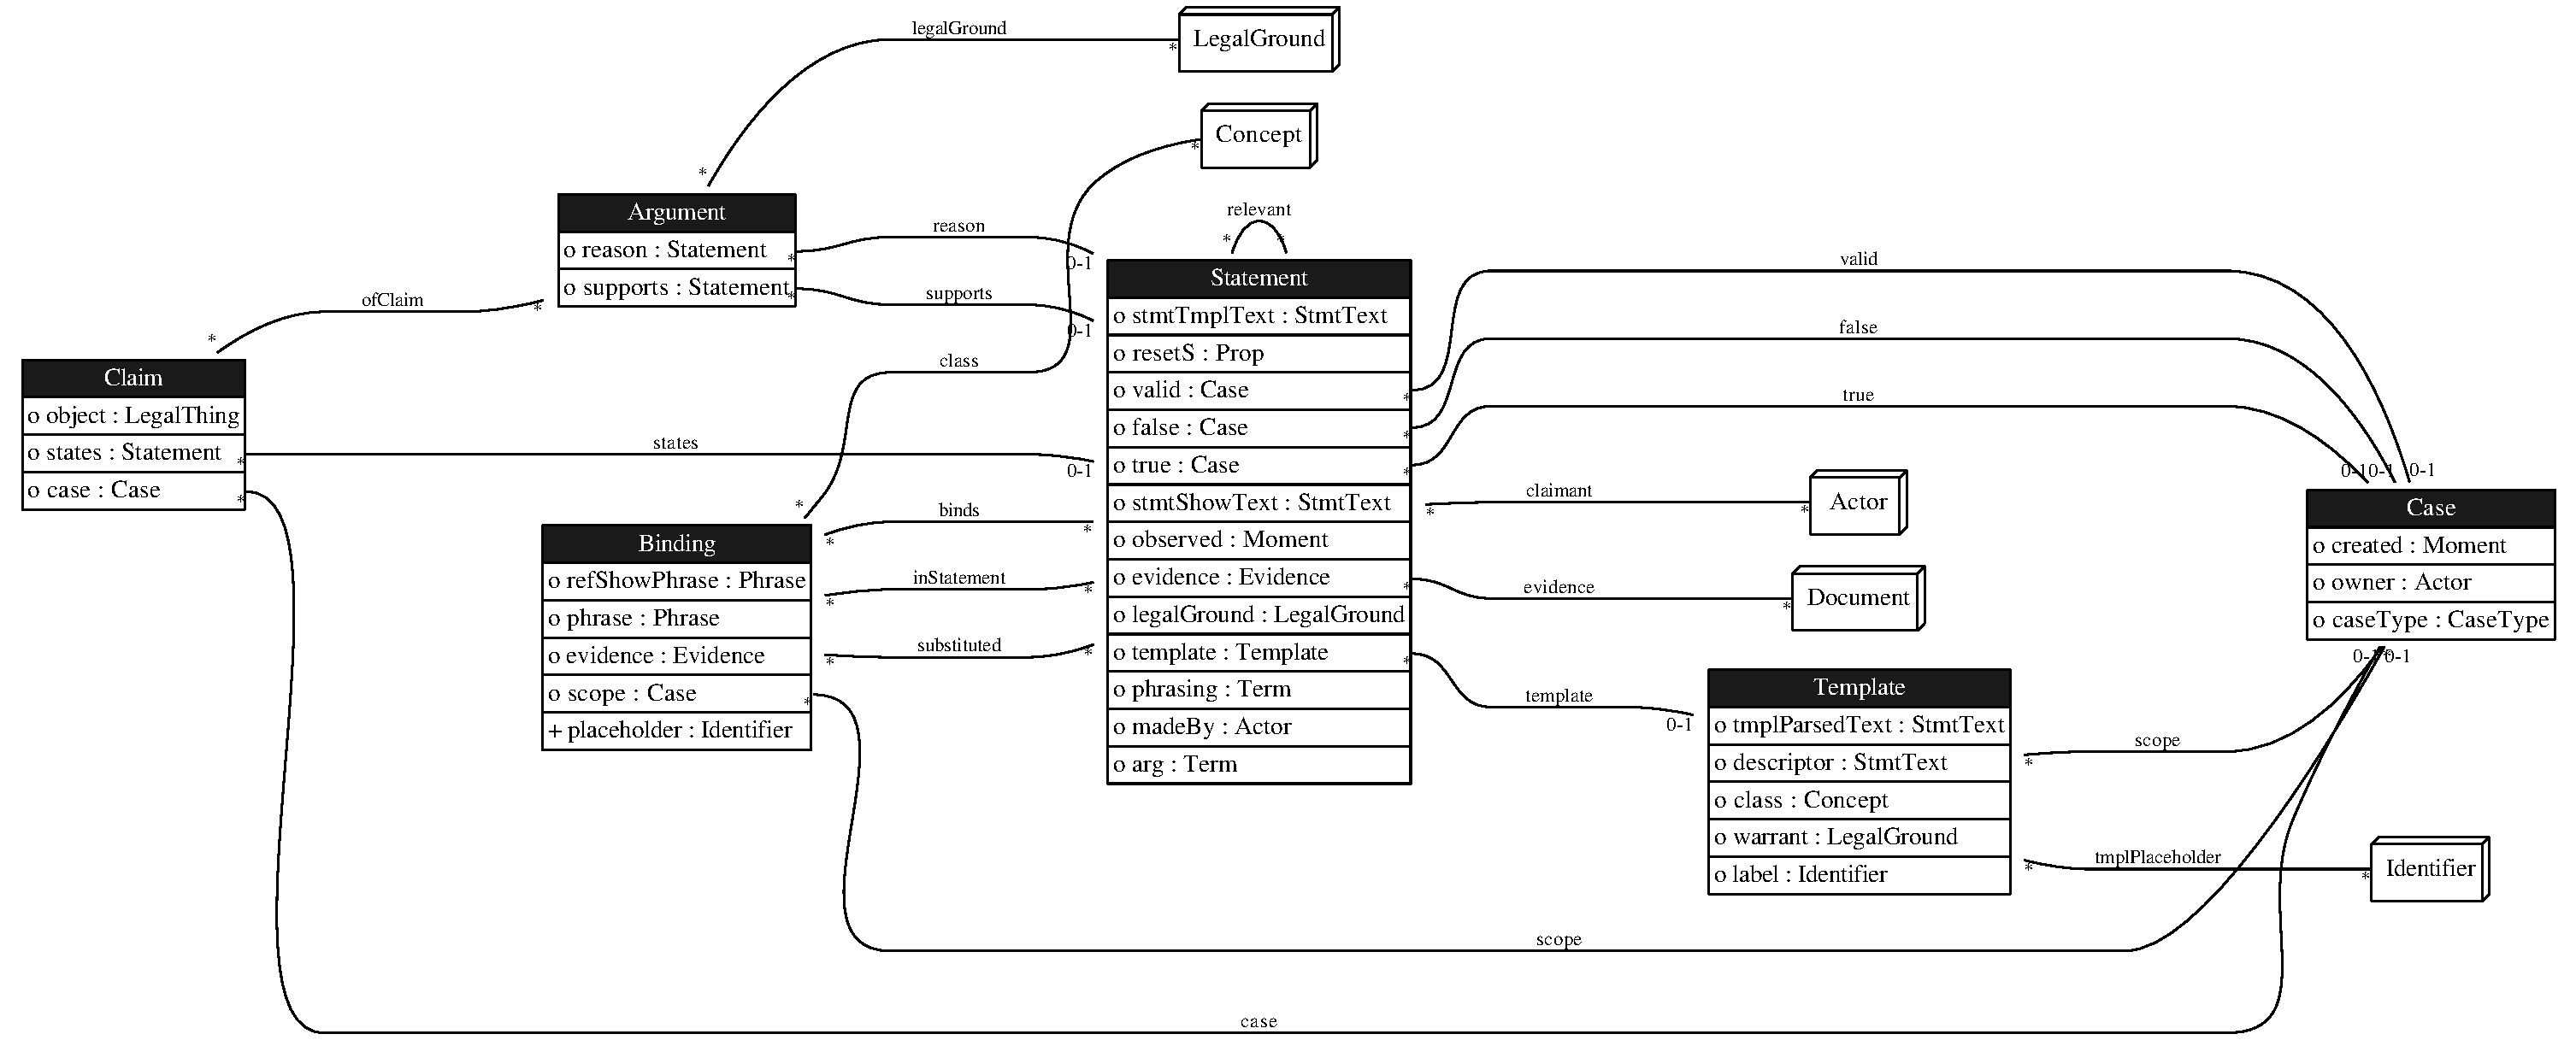
\includegraphics[scale=.23]{LogicalDataModel.pdf}
\end{center}
\caption{Conceptual data model}
\label{fig:conceptual model}
\end{figure}
	
	To convey the flavour of software development in relation algebra, it suffices to discuss a tiny part of the whole program.
	Therefore, we shall discuss the part of the conceptual model that is used in the sequel.
	The context in which a user creates arguments and reasons about them is a legal case.
	For this reason, validity, falsehood and truth of statements are related to the case.
	A \define{statement} is a phrase in natural language that can be either true or false.
	An example is \stmtText{The employee, John Brown, is entitled to 50 Euros}%
\footnote{This type of statement is typical for cases. It is valid only in the case where this particular John Brown is known.
	In other cases, where John Brown is unknown, this statement is meaningless}.
	In MirrorMe, a user can define a template, such as \stmtText{The employee, [emp], is entitled to [increase]}.
	The strings \stmtText{[emp]} and \stmtText{[increase]} are called placeholders.
	The reason for using placeholders is that legal rules are stated in general terms, e.g.
	\stmtText{Every employee is entitled to an increase in salary}.
	The user of MirrorMe will pick a legal text (from a source he trusts) and substitute parts of that text by placeholders.
	When the facts are known, the argument can be completed by substituting placeholders by actual phrases.

	It is precisely this substitution process that we have chosen to describe in this paper as a case study in
	programming with relation algebra.

\section{Programming in Relation Algebra}
\label{sct:Programming in RA}
	At this point we have reached the core of this case study.
	We focus on the substitution of placeholders when their values change.
	By focusing on this tiny detail, we can discuss the mechanics ``under the hood'' of the application generated by Ampersand.

	First we show how the computer solves the issue by looking at an exerpt of a log file (figure~\ref{fig:log file}).
	It shows an alternating sequence of the computer (ExecEngine) mentioning a rule,
	followed by insert or delete actions to satisfy that rule.
	Then we zoom in further, one rule at a time, to explain precisely what each rule looks like and how programming is done.
	We then discuss the same flow of events by means of a graph (figure~\ref{fig:event flow}) in which these rules and actions are nodes.
	This graph serves as an event flow diagram to illustrate the process behind figure~\ref{fig:log file}.

\begin{figure}[htb]
\begin{verbatim}
 ExecEngine run started
 ExecEngine satisfying rule 'signal phrase update'
 InsPair(resetS,Statement,Stat623,Statement,Stat623)
 ExecEngine satisfying rule 'flush substitutions'
 DelPair(substituted,Binding,Bind625,Statement,Stat623)
 ExecEngine satisfying rule 'reset statement text'
 InsPair(stmtShowText,Statement,Stat623,StmtText,
         The employee, [emp], is entitled to [increase].)
 ExecEngine satisfying rule 'done initializing'
 DelPair(resetS,Statement,Stat623,Statement,Stat623)
 ExecEngine satisfying rule 'substitute'
 InsPair(stmtShowText,Statement,Stat623,StmtText,
         The employee, James, is entitled to [increase].)
 InsPair(substituted,Binding,Bind625,Statement,Stat623)
 ExecEngine satisfying rule 'fill shownPhrase'
 InsPair(shownPhrase,Binding,Bind625,Phrase,James)
 ExecEngine run completed
\end{verbatim}
\caption{Log file of a substitution}
\label{fig:log file}
\end{figure}
	The log file of figure~\ref{fig:log file} has been taken from a computer that carries out the procedure to satisfy all rules.
	The machine will only act on rules that are violated.
	The first rule to be violated is ``signal phrase update'', in which the computer signals that something or someone has made a change
	in relation \id{phrase}.
	The procedure ends by doing the necessary substitutions,
	ensuring that all statements have the actual phrase of a placeholder in their text.

	Let us now study the actual rules to see how these rules cause the right actions to take place in the correct order.
	We will follow the log file from figure~\ref{fig:log file} in reverse direction,
	reasoning backwards from the result.

	Whether a placeholder has been edited can be observed by comparing its new phrase to the shown phrase%
\footnote{Note that we use the notion ``the phrase of a placeholder'' to indicate a pair from $\flip{\id{phrase}};\id{placeholder}$.}.
	The phrase of a placeholder is kept in the relation \id{phrase}.
	The shown phrase is kept in the relation \id{shownPhrase}.
	The sole purpose for having the relation \id{shownPhrase} is to detect a change in \id{phrase}.
	Let us introduce \id{differB} to represent the bindings with an updated phrase:
\[\id{differB} = \ident{Binding}\cap\id{shownPhrase};\cmpl{\ident{Phrase}};\flip{\id{phrase}}\]
	When the phrase of a placeholder changes,
	that phrase must be updated in every statement in which the placeholder was used.
	That update action is specified in section~\ref{rule: substitute}.
	Section~\ref{rule: fill shownPhrase} specifies how \id{shownPhrase} is made equal to \id{phrase},
	after all necessary substitutions are done.

\subsection{rule: fill shownPhrase}
\label{rule: fill shownPhrase}

\[\text{RULE}\ (\ident{Binding}\cap\id{substituted}/\id{inStatement} );\id{phrase}\ \subs\ \id{shownPhrase} \]
        This rule says that for each binding that has been substituted in every statement it is used in,
	the \id{phrase} must be equal to the \id{shownPhrase}.
	When violated, it is satisfied by inserting all violations into \id{shownPhrase}.

\subsection{rule: substitute}
\label{rule: substitute}
	Let us now look into the process of substituting placeholders by phrases.
	The relation \id{tmplParsedText} contains the original text, provided by a user.
	Placeholders are specified by enclosing them in brackets,
	e.g. \stmtText{The employee, [emp], is entitled to [increase]}.
	The text in which a placeholder has been substituted by a phrase,
	e.g. \stmtText{The employee, John Brown, is entitled to 50 Euros},
	is kept in relation \id{stmtShowText}.
	Each substitution that has been done in a statement corresponds to a binding-statement pair in the relation \id{substituted}.
	This relation keeps track of all substitutions.
	After a placeholder has been substituted, it no longer occurs in \id{stmtShowText}.
	This poses a problem if we want to substitute the new phrase in \id{stmtShowText}.
    For the placeholder that defines the place in the text where to substitute, is no longer in that text.
	Therefore, substitutions must be done in the original text of the statement.
	All placeholders in that text must then be substituted again.
	So, the text in \id{stmtShowText} must first be reset to the original text from \id{tmplParsedText}.
	To keep track of substitutions correctly, all corresponding binding-statement pairs must be removed from the relation \id{substituted}.
	Only after resetting is done, the substitutions can be put back in place with the new phrases filled in.
	
	We define a relation \id{resetS} to register the statements that are being reset.
    In statements that are not being reset, $\ident{Statement}-\id{resetS}$, substitutions can take place.
	All placeholders that have a binding with a phrase can be substituted. 
	The following rule specifies the action of substituting placeholders.
\begin{displaymath}
\begin{array}{rl}
\multicolumn{2}{l}{\text{RULE}}\\
&(\ident{Binding}\cap \id{phrase} ;\flip{\id{phrase}});\id{inStatement} ;(\ident{Statement} - \id{resetS})\\
\subs\\
&\id{substituted}
\end{array}
\end{displaymath}
	Violations of this rule are binding-statement pairs, of which the binding has a phrase and the statement is not being reset.
	Hence, this rule can be satisfied by inserting every violation into the relation substituted.

\subsection{rule: done initializing}
\label{rule: done initializing}
	Resetting a statement is done when two conditions are met.
	First, every statement that is (still) being reset may have no bindings in the relation \id{substituted}.
	Second, the text in \id{stmtShowText} corresponds to the text in \id{tmplParsedText}.
	So the rule that specifies the action is:

\begin{displaymath}
\begin{array}{rl}
\multicolumn{2}{l}{\text{RULE}}\\
&(\id{resetS} - \flip{\id{inStatement}};\id{substituted})\ \cap\\
&\id{template} ;\id{tmplParsedText} ;\flip{\id{stmtShowText}}\\
\subs\\
&\overline{\id{resetS}}
\end{array}
\end{displaymath}
	Violations of this rule are statements that are no longer being reset, but are still in the relation \id{resetS}.
	The appropriate action is to remove them from \id{resetS}.

\subsection{rule: reset statement text}
\label{rule: reset statement text}
	To satisfy one condition from section~\ref{rule: done initializing},
	the text in \id{stmtShowText} must be made equal to the original text in the template.
	The action is specified by the following rule:
\[\text{RULE}\ \id{resetS} ;\id{template} ;\id{descriptor}\ \subs\ \id{stmtShowText} \]
	Violations of this rule are descriptors of templates that belong to statements that are being reset.
	These violations can be resolved by inserting them in \id{stmtShowText}.

\subsection{rule: flush substitutions}
\label{rule: flush substitutions}
	To satisfy the other condition from section~\ref{rule: done initializing},
	the following rule specifies the action to be taken:
\[\text{RULE}\ \fullt{Binding}{Binding};\id{inStatement} ;\id{resetS}\ \subs\ \overline{\id{substituted} }\]
	Every binding in a statement that is being reset needs to be removed from the relation \id{substituted}.
	The software developer can implement this by deleting all violations of this rule from the relation \id{substituted}.

\subsection{rule: signal phrase update}
\label{rule: signal phrase update}
	When the phrase in a binding is edited and the new phrase differs from the shown phrase,
	this signals that substitutions must be flushed (see~\ref{rule: flush substitutions}),
	that the statement text must be reset to the original text (see~\ref{rule: reset statement text}),
	that the reset-state must be revoked (see~\ref{rule: done initializing}),
	that substitution must take place (see~\ref{rule: substitute}),
	and finally that the phrase detection is switched off again (see~\ref{rule: fill shownPhrase}).
	The initial condition occurs if a binding has been used (substituted) in a statement,
	and the binding satisfies \id{differB}.
	The following rule specifies the action that resetting a statment can start:
\[\text{RULE}\ \ident{Statement}\cap \flip{\id{inStatement}};\id{{\it differB}};\id{substituted}\ \subs\ \id{resetS} \]
	Violations of this rule are statements of which a substitution must be re-done.
	The software developer can have these violations added to \id{resetS} to satisfy this rule.
	In doing so, the chain of events is triggered that ends when all rules are satisfied.

\section{Programming in the Small}
\label{sct:Programming}
	Let us take a closer look at the programming process.
	Working in relation algebra, a software developer must think about satisfying constraints.
	She considers how violations arise from changing content of relations.
	And she thinks about insert and delete actions to restore these violations.
	In our case study, we have reasoned with the event types: Ins $\la\id{relation}\ra$ and Del $\la\id{relation}\ra$%
\footnote{Ins and Del are called each others duals.}.
\begin{table}[htb]
{\small\begin{tabular}{|l|p{3.3in}|}\hline
rule&event types\\ \hline
signal phrase update&\small Ins \id{inStatement}, Ins \id{differB}, Ins \id{substituted}, Del \id{resetS}\\
flush substitutions&\small Ins \id{inStatement}, Ins \id{resetS}, Del \id{substituted}\\
reset statement text&\small Ins \id{resetS}, Ins \id{template}, Ins \id{descriptor}, Del \id{stmtShowText}\\
done initializing&\small Ins \id{resetS}, Del \id{inStatement}, Del \id{substituted}, Ins \id{template}, Ins \id{tmplParsedText}, Ins \id{stmtShowText}\\
substitute&\small Ins \id{phrase}, Ins \id{inStatement}, Del \id{resetS}, Del \id{substituted}\\
fill shownPhrase&\small Ins \id{substituted}, Del \id{inStatement}, Del \id{shownPhrase}, Ins \id{phrase}\\ \hline
\end{tabular}}
\caption{By which type of events can rules be violated?}
\label{fig:violation of rules}
\end{table}
	Table~\ref{fig:violation of rules} shows which event types may violate which rules.
	Recall section~\ref{sct:Programming in RA}, where the process of substitution started by updating the value of a placeholder.
	This meant doing an insert after a delete on the relation \id{phrase}, causing the updated phrase to appear in \id{differB}.
	That was signaled by the rule ``signal phrase update''.
\begin{figure}[bht]
\begin{center}
  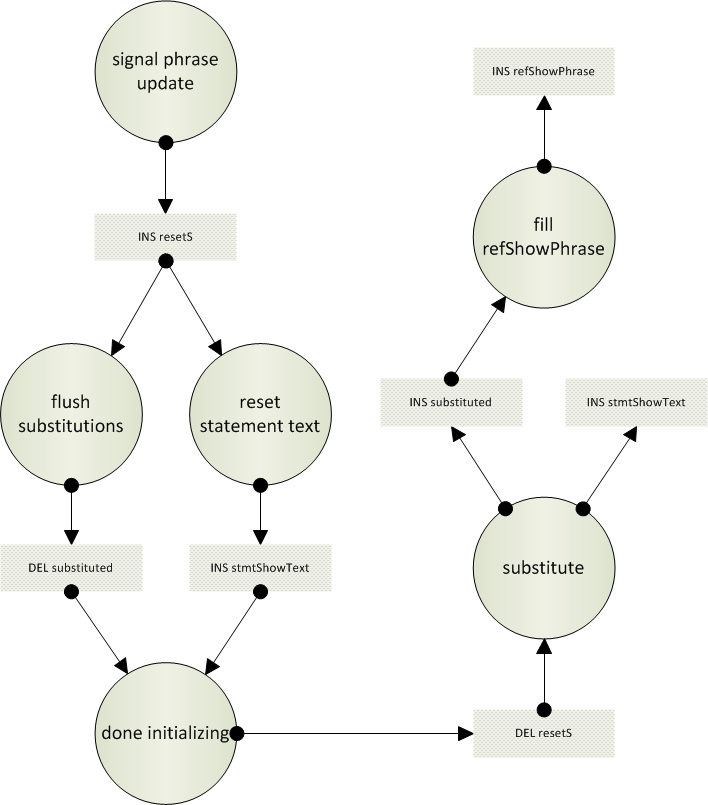
\includegraphics[scale=.55]{eventFlow.png}
\end{center}
\caption{event flow}
\label{fig:event flow}
\end{figure}
	In general, the software developer must decide how to resolve violations that occur as a result of some event.
	This can be done by choosing among the duals of the event types from table~\ref{fig:violation of rules}.
	By systematically swapping Ins for Del and vice-versa,
	the table shows by which type of events violations can be restored.
	To ensure progress, the software developer will pick a different relation for restoring than the relation that causes the violation.
	The software developer can draw a graph that contains all information from table~\ref{fig:violation of rules}
	and the dual information.
	Figure~\ref{fig:event flow} shows part of that graph.
	A circle represents a rule, a rectangle represents an event type, and the arrows connect them.
	The software developer can work her way through the graph, to write code to restore invariants for every event type that might cause violations.
	Figure~\ref{fig:event flow} shows just that part of the graph that corresponds with the case study in this article.

\section{Reflection}
\label{sct:Reflection}
	Ampersand is built on the belief that software development should be automated.
	It uses rules to represent requirements, in the firm belief that consistent requirements are essential to the software development process~\cite{Boehm1981}.
	Being fully aware of the fate of formal methods in computer science, Ampersand is founded on the belief that software development must be done more formally.
	So Ampersand is building further on the foundations laid by formal specification methods
	such as Z~\cite{Z} and Alloy~\cite{Alloy2006}.
	In contrast however with such methods, Ampersand is equipped with a software generator that generates an information system.
	Thus, specifying in Ampersand is developing software at the same time.
	Ampersand complements the RelView approach~\cite{Berghammer2005}, which also generates software but is stronger in specifying complex computational problems.

	In retrospect we see that programming in relation algebra yields an unconventional programming experience.
	This experience consists of inventing rules and choosing event types for resolving violations, as illustrated by the case study.
	To relate this experience to programming as we know it, section~\ref{sct:Comparison} makes a comparison with established programming languages (prior art).
	Section~\ref{sct:Contribution} summarizes the contributions to software development claimed by Ampersand.
	Section~\ref{sct:Ampersand in practice} summarizes the use of Ampersand in practice and
	section~\ref{sct:Further Research} gives an outlook on research that is required in the near future.

\subsection{Comparison}
\label{sct:Comparison}
	This section compares Ampersand with existing programming paradigms by mentioning the most important differences and similarities.

	The first to compare with is the imperative programming paradigm, known from popular languages such as Java~\cite{Java} and C++~\cite{Stroustrup97a}.
	Our case study cannot be called imperative, because the notion of control flow in imperative languages is very different.
	In imperative languages, the control flow is defined by the software developer.
	In this case study, the control flow emerges as a result of changes in relation content as illustrated
	by figure~\ref{fig:event flow}.

	The case study also differs from the logic programming paradigm of Prolog~\cite{Lloyd1984} and of all rule engines that can be considered to be an offspring of Prolog.
	A difference lies in the way rules are interpreted.
	In logic programming, a program consists of Horn-clauses and a resolution-proof is constructed on run-time.
	The software developer works with notions such as backtracking (backward chaining) and unification, which are absent in Ampersand.
	Ampersand is not restricted to Horn-clauses; any relation-algebraic equation over relations can be used as a rule.

	The case study also differs from functional programming, of which Haskell and Scala are prominent representants.
	A core idea in functional programming is to evaluate a program as a function from input to output~\cite{Backus1978}.
	A functional program consists of function definitions, that are evaluated by a term- or graph-rewriter, using various strategies such as lazy or eager evaluation.
	In contrast, one might interpret our case study as a relaxation of the constraint that everything is a function.
	In relation algebra, everything is a relation and a function is a restricted form of a relation.
	A similarity to functional programming is the declarative style, because substitution of equal terms without changing the semantics is a property we see in both worlds.

	A difference with database programming is found in the type of algebra that is used.
	Relational databases are founded on relational algebra~\cite{Codd70}. They are typically programmed in SQL.
	In contrast with database programming, Ampersand implements heterogeneous relation algebra~\cite{Schmidt1997}.
	A software developer working with relational algebra sees n-ary tables, while Ampersand is restricted to binary relations.
	The comparison between relation{\it al} algebra and relation algebra might relate to comparing relational databases with graph databases~\cite{Vicknair2010},
	although no literature was found to corroborate this.

	In the tradition of formal specification, there are many relational approaches, such as Z~\cite{Z}, CSP~\cite{CSP}, LOTOS~\cite{LOTOS}, VDM~\cite{VDM}.
	Where formal specification techniques typically analyse and diagnose specifications,
	Ampersand actually synthesizes (generates) information systems.

	If Ampersand represents a programming style at all, we might call it ``a relation-algebraic style of programming''.
	That style would be characterized by a programmer who specifies constraints and a computer trying to satisfy these constraints by resolving violations.

\subsection{Contribution}
\label{sct:Contribution}
	Contributions of Ampersand to the software development process are:
\begin{itemize}
\item	Ampersand has the usual benefits of a declarative language:
	This means that terms can be manipulated by Tarski's axioms without changing their semantics~\cite{vdWoude2011}.
	It also means that the order in which rules are written has no consequence for their semantics.
\item	Heterogeneous relation algebra has a straightforward interpretation in natural language~\cite{RBD}.
	We have used that to formalize business requirements without exposing business stakeholders to any formal notation.
\item	Heterogeneous relation algebra in Ampersand is statically typed~\cite{Joosten2015}.
	There is much evidence for significantly lower software maintenance cost due to static typing as opposed to dynamic typing~\cite{HanenbergKRTS14,Petersen2014}.
\item	Heterogeneous relation algebra is well studied.
	As a consequence, many tools that are readily available in the public domain can be put to good use.
	For executives of large organizations it can be reassuring that the formalism is free of childhood diseases.
\item	Relation algebra facilitates composing software from reusable components, because a program consists of rules.
	Since the union of sets of rules is a set of rules, compositionality comes from the union operator.
	In practice, when components are brought together in larger assemblies, hardly any adjustments have to be made%
\footnote{This is (unsubstantiated) experience collected from projects we have done with Ampersand.}.
\end{itemize}

	Ampersand also has disadvantages. It appears to be difficult to learn for large groups of software professionals.
	Research~\cite{Michels2015} shows that this is largely due to deficits in prerequisite knowledge, especially skills in discrete mathematics.
%	For this reason, we have made an addendum to the course we teach at the Open University of the Netherlands.
	Also, programming appears to be difficult in practice.

\subsection{Ampersand in Practice}
\label{sct:Ampersand in practice}
	Ampersand has been used in practice both in education (Open University of the Netherlands)
	and in industry (Ordina and TNO-ICT).
	For example, Ordina designed a proof-of-concept in 2007 of the INDIGO-system.
	This design was based on Ampersand, to obtain correct, detailed results in the least amount of time.
	Today INDIGO is in use as the core information system of the Dutch immigration authority, IND.
	More recently, Ampersand was used to design an information system called DTV for the Dutch food authority, NVWA.
	A prototype of DTV was built in Ampersand and was used as a model to build the actual system.
	TNO-ICT, a major Dutch industrial research laboratory, is using Ampersand for research purposes.
	For example, TNO-ICT did a study of international standardizations efforts such as
	RBAC (Role Based Access Control) in 2003 and architecture (IEEE 1471-2000)~\cite{IEEE1471} in 2004.
	Several inconsistencies were found in the last (draft) RBAC standard~\cite{RBAC}.
	TNO-ICT has also used the technique in conceiving several patents%
\footnote{e.g. patents DE60218042D, WO2006126875, EP1727327, WO2004046848, EP1563361, NL1023394C, EP1420323, WO03007571, and NL1013450C.}.
	At the Open University of the Netherlands, Ampersand is being taught in a course called Rule Based Design~\cite{RBD}.
	In this course, students use a platform called RAP, which has been built in Ampersand~\cite{Michels2015}.
	RAP has been the first Ampersand-application that has run in production.

\subsection{Further Research}
\label{sct:Further Research}
	Further research on this topic is required to bring relation algebra still closer to the community of practitioners.
	Further use of relation algebra can be made by incorporating a model checker, such as the Alloy analyser~\cite{Alloy2006}, to detect inconsistent rules.
	An exciting new development is Amperspiegel~\cite{Amperspiegel}, which brings notational flexibility at the fingertips of the user.
	Developments in the Ampersand-compiler are going towards a rule-repository (written in Ampersand itself).
	This will make collaborative information systems development in Ampersand easier, because the repository can assist in automating
	the software development process further.
	Other research is needed towards a comprehensive theory of information systems.
	Currently, there is no theory (in the mathematical meaning of the word) for information systems.
	In the Ampersand project, a sub-project called ``Formal Ampersand'' is being conducted to achieve this goal.
\bibliographystyle{spmpsci}
\bibliography{doc}


\end{document}
